\documentclass{standalone}
\usepackage{tikz}
\usetikzlibrary{matrix, positioning,calc,arrows.meta, backgrounds,fit}
\usepackage[dvipsnames]{xcolor}
\usetikzlibrary{shapes.geometric}
\tikzset{
    every node/.style={font=\small},
    rectred/.style={draw=red, fill=green!80!black!10, thick, rounded corners,  align=center},
    rectblue/.style={  rounded corners, align=center},
    yellowbox/.style={draw=black, fill=Dandelion, thick, rounded corners, align=center},
    greencycle/.style={fill=green!80!black!10,ellipse, align=center},
    bluecycle/.style={fill=NavyBlue, ellipse, align=center},
    arrow/.style={-{Latex[length=3mm]}, thick},
}
\begin{document}
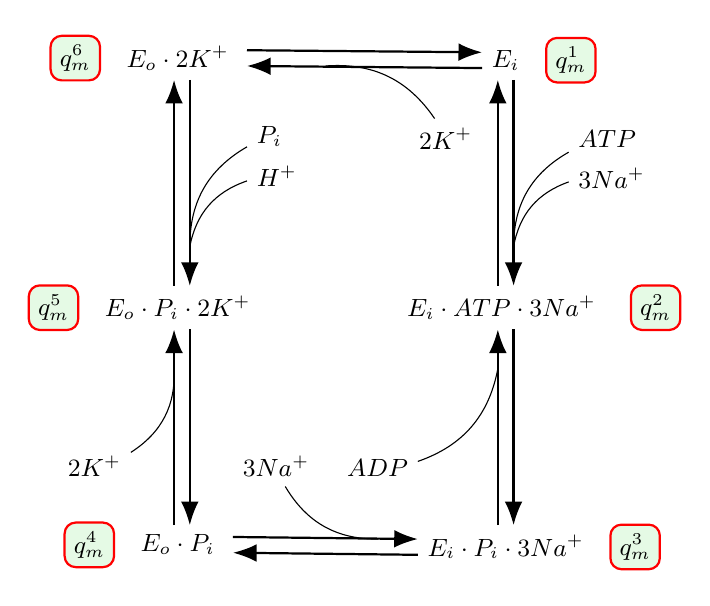
\begin{tikzpicture}[node distance=15mm and 0mm]
% Define the row width (distance between start and end nodes)
\def\rowwidth{60mm}
\def\sep{25mm}
\def\sepp{30mm}
% width of the side bands (change as you like)
\def\bandwidth{22mm}
\matrix (top) [matrix of nodes,column sep=\sepp] {
  |[rectblue]| $E_o\cdot 2K^+$ &  |[rectblue]| $E_i$\\  
};

\foreach \col/\text in {1/$q_m^{6}$}{
  \node[rectred,left=2mm of top-1-\col] (top2-\col) {\text};
}

\foreach \col/\text in {2/$q_m^{1}$}{
  \node[rectred,right=2mm of top-1-\col] (top2-\col) {\text};
}

\matrix (left) [matrix of nodes,row sep=\sep, matrix anchor=north, below=\sep of top-1-1]  {
 |[rectblue]| $E_o\cdot P_i\cdot 2K^+$ \\ 
 |[rectblue]| $E_o\cdot P_i$  \\ 
};

\foreach \row/\text in {1/$q_m^{5}$, 2/$q_m^{4}$}{
  \node[rectred,left=2mm of left-\row-1] (left2-\row) {\text};
}

\matrix (right) [matrix of nodes,row sep=\sep, matrix anchor=north, below=\sep of top-1-2]  {
  |[rectblue]| $E_i\cdot ATP\cdot 3Na^+$ \\ 
  |[rectblue]| $E_i\cdot P_i\cdot 3Na^+$\\ 
};

\foreach \row/\text in {1/$q_m^{2}$, 2/$q_m^{3}$}{
  \node[rectred,right=2mm of right-\row-1] (right2-\row) {\text};}

% 2 K+ binding on the left side of left-1-1 and left-2-1
\node [rectblue, left=of left-2-1, yshift=10mm] (K2) {$ 2K^+$};
\draw[bend right] (K2) to ([xshift=-1mm,yshift=-5mm]left-1-1.south);

% Pi and H+ release on the right side of top-1-1
\node [rectblue, right=of top-1-1, yshift=-10mm] (Pi) {$ P_i $};
\node [rectblue, right=of top-1-1, yshift=-15mm] (H) {$ H^+ $};
\draw[bend right]  (Pi) to ([xshift=1mm,yshift=5mm]left-1-1.north);
\draw[bend right] (H) to ([xshift=1mm,yshift=5mm]left-1-1.north);

\node [rectblue, left=of top-1-2, yshift=-10mm] (K2_i) {$ 2K^+$};
\draw[bend right] (K2_i) to ([xshift=10mm,yshift=-1mm]top-1-1.east);

\node [rectblue, right=of top-1-2, xshift=5mm,yshift=-10mm] (ATP) {$ ATP$};
\node [rectblue, right=of top-1-2, xshift=5mm,yshift=-15mm] (Na) {$ 3Na^+$};
\draw[bend right]  (ATP) to ([xshift=1mm,yshift=5mm]right-1-1.north);
\draw[bend right] (Na) to ([xshift=1mm,yshift=5mm]right-1-1.north);

\node [rectblue, left=of right-2-1, yshift=10mm] (ADP) {$ ADP$};
\draw[bend right] (ADP) to ([xshift=-1mm,yshift=-5mm]right-1-1.south);

\node [rectblue, right=of left-2-1, yshift=10mm] (Na_o) {$ 3Na^+$};
\draw[bend right] (Na_o) to ([xshift=-5mm,yshift=1mm]right-2-1.west);

\draw[arrow] ([xshift=-1mm]left-1-1.north) -- ([xshift=-1mm]top-1-1.south);
\draw[arrow] ([xshift=-1mm]left-2-1.north) -- ([xshift=-1mm]left-1-1.south);
\draw[arrow] ([xshift=-1mm]right-1-1.north) -- ([xshift=-1mm]top-1-2.south);
\draw[arrow] ([xshift=-1mm]right-2-1.north) -- ([xshift=-1mm]right-1-1.south);

\draw[arrow] ([xshift=1mm]top-1-1.south) -- ([xshift=1mm]left-1-1.north);
\draw[arrow] ([xshift=1mm]left-1-1.south) -- ([xshift=1mm]left-2-1.north);

\draw[arrow] ([xshift=1mm]top-1-2.south) -- ([xshift=1mm]right-1-1.north);  
\draw[arrow] ([xshift=1mm]right-1-1.south) -- ([xshift=1mm]right-2-1.north);

\draw[arrow] ([yshift=1mm]top-1-1.east) -- ([yshift=1mm]top-1-2.west);
\draw[arrow] ([yshift=-1mm]top-1-2.west) -- ([yshift=-1mm]top-1-1.east);

\draw[arrow] ([yshift=1mm]left-2-1.east) -- ([yshift=1mm]right-2-1.west);
\draw[arrow] ([yshift=-1mm]right-2-1.west) -- ([yshift=-1mm]left-2-1.east);

\end{tikzpicture}
\end{document}
